\documentclass{article}
\usepackage[utf8]{inputenc}
\usepackage{hyperref}
\title{keccak preimage}
\usepackage{graphicx}
\usepackage{tikz}
\usepackage{tikz,graphicx}
\usepackage[absolute,overlay]{textpos} 
\usetikzlibrary{decorations.pathmorphing,matrix,decorations.pathreplacing,arrows,decorations.markings}
\usetikzlibrary{fit,calc,shapes,arrows,positioning,shadings,backgrounds,patterns,tikzmark,matrix,spy}
\usetikzlibrary{decorations.markings}

\usepackage[T1]{fontenc}
\begin{document}

\maketitle

\section{Introduction}

The observations based on the following paper : \textbf{Linear Structures: Applications to Cryptanalysis of Round-Reduced Keccak}.

\subsection{2R Keccak-512}

See Fig. 8, for each guess :
we set 
\[
    A[0, 1] = A[0, 0] \oplus \alpha_{0}
\]
\[
    A[2, 1] = A[2, 0] \oplus \alpha_{2}
\]
with $\alpha_0$ and $\alpha_2$ as random constants

Since $A[0,0]$ and $A[2,0]$ have 128 bits. So we have a complexity gain over bruteforce of $2^{128}$. Hence the time complexity $= 2^{512 - 128} = 2^{384}$.

Input degree of freedom : 
\begin{enumerate}
    \item 64 bits from $A[0, 0]$ , 64 bits from $A[2,0]$.
    \item (320 -1) bits from white lanes
    \item 128 bits from $\alpha_0, \alpha_2$
\end{enumerate}

This sums upto 575 bits larger than required 512 bits.

\subsection{2R Keccak-384}

\begin{enumerate}
    \item Attack similar to Keccak-512
    \item Can obtain a linear structure of 256 bits variables from 
    \[
        (A[0, 0], A[0, 1], A[2, 0], A[2, 1])
    \]
    
    \item with : $A[0, 2] = A[0, 0] \oplus A[0, 1] \oplus \alpha_0$
    \item and $A[2, 2] = A[2, 0] \oplus A[2, 1] \oplus \alpha_2$
    \item Hence a linear system of 256-bit equations
    \item Msg satisfying padding rule, need a solution with the last bit of A[2,2] being 1
    \item Time Complexity of Attack $ = 2^{384 - 256 + 1} = 2^{129}$
\end{enumerate}

\textbf{Note :} In the following document WM refers to Willi Meier

\section{Suggestion by WM}

\subsection{Mail : 5 Feb}

Mail contents are : 
\begin{quote}
    I mainly refer to : https://eprint.iacr.org/2016/878
    
    We try to loosen restrictions imposed by linear structures to increase freedom degrees.
    
    An example is 2-round Keccak-384. I refer to Fig. 9. In addition to the colored 6 lanes that are variable, we also keep lanes 3,0 and 3,1 variable, still so that sum of columns is kept constant. Then $\chi$ produces one quadratic lane. We substitute quadratic monomials by 64 linear variables.
    
    We can invert the first row of image (green), and we require that the map to the 6-th green lane is linear (i.e. quadratic part happens to vanish). The probability for this event is about $.75^{64} = 2^{27}$

    Then we have $ 4*64 + 64 + 64 = 384$ variables and the same number of conditions. Solving this linear system has about 1 solution, that we may check by substituting it into 2-round Keccak. Genuine number of freedom degrees is 320, and artficial ones 384. It is likely to find a correct solution in $2^{64} * 2^{27}= 2^{91}$ trials. This case was found in discussion with Meicheng Liu and Jian Guo.
    I believe that something similar (or better) will work for 2-round Keccak-512. In addition to substitution of a quadratic lane by linear variables, we know that variables in same column are linearly related. This means that in quadratic lanes after $\chi$, some linear factors  are essentially "the same".

    The probability of a1*a2 =a1*a3 is 0.75 for any values a1, a2, a3. We substitute monomials of the form a1*a2  and a1*a3 by the same linear variable to get more linear equations that will hold true with reasonable probability. We introduce artificial linear variables economically, so that we don't have more linear variables (genuine and artificial ones) than equations.Details need to be checked.
    
    Wonder whether this could also help, e.g., in 3-round Keccak-256 in \url{https://tosc.iacr.org/index.php/ToSC/article/view/802}.
    
    An issue is how far these observations extend to improve 3 round preimages of Keccak-384 and Keccak-512, as described in Sect. 6.3.
    
    As complexities of known preimages of 4-round Keccak-512 are still close to $2^{512}$, there is some slight hope that we might reach 4 rounds for this case.
    
    Do you have any comments on this?
    \end{quote}
    
    \begin{enumerate}
        \item Here in addition to Keccak-384 setting for 2 Round attack.
        \item In Fig. 9 we keep lanes (3, 0) and (3, 1) also as variables
        \item $A[3, 1] = A[3, 0] \oplus \alpha_3$ (so that sum of columns remains constant)
        \item Linear structure of 320-bit :
        \item $( A[0, 0], A[0, 1], A[2, 0], A[2, 1], A[3, 0] )$
        \item A quadratic term is introduced after 1st $\chi$ by product of $(2, 0), (3, 1)$ as both are variables.
        \item For this we substitute quadratic monomials by 64 linear variables.
        \item Now next problem was for last round : $(\chi o \iota)^{-1}$
        \item For the green lane of second row, this happens to be linear with probability $= 0.75$
        \item For 64 slices, this $= 0.75^{64}$, which adds $2^{27}$ trials
        \item Complexity comes out to be $ = 2^{64} * 2^{27} = 2^{91}$ trials.
        \item \textbf{ Comments : }
        \begin{enumerate}
            \item Any issue of Linear independent variable for solution of equations?
            \item Otherwise the analysis is fine here.
        \end{enumerate}
    \end{enumerate}
    \subsection{Suggestion for Keccak-384, 2R}
\begin{enumerate}
    \item \textbf{Note :} After verification this comes out to be incorrect
    \item Same as the setting introduced by WM for 2R Keccak-384 where we keep (3,0) and (3,1) also as variables
    \item Here we introduced a new variable for each quadratic term
    \item The suggestion here is for reducing the trials due to the last round linear $\chi$ inversion.
    \item Instead of inverting $\chi$ for 6th green lane as suggested by WM we can do something like this :
    \item \label{ob2}\textbf{Observation :} When only one output bit is known after $\chi$ step, then the corresponding input bits have $2^4$ possibilities. A way to fix the first output bit to be the same as input bit and the second bit as $1$. It is shown in the Figure~\ref{chi_inv2}.
\begin{figure}[ht]
\begin{center}
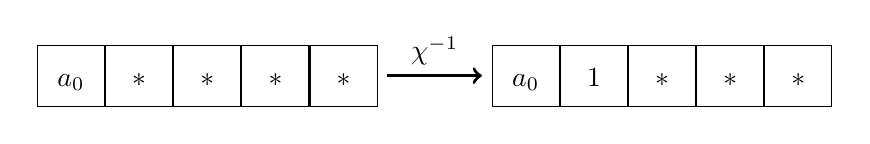
\begin{tikzpicture}[ampersand replacement=\&]
\matrix (m1) [matrix of nodes,
nodes={inner sep=5pt,text width=0.5cm,align=center,minimum height=.5cm, draw,text height=1em,text depth=.2em}
]{
	$a_0$ \& $*$ \& $*$ \& $*$ \& $*$\\
};

\matrix (m2) [right = 1.2cm of m1, matrix of nodes,
nodes={inner sep=5pt,text width=0.5cm,align=center,minimum height=.5cm, draw,text height=1em,text depth=.2em}
]{
	$a_0$ \& $1$ \& $*$ \& $*$ \& $*$\\
};
\draw[->, very thick] (m1)-- node[above, pos=0.5] {$\chi^{-1}$} (m2);
\end{tikzpicture}
\end{center}
\caption{Computation of $\chi^{-1}$\label{chi_inv2}}
\end{figure}
    \item Here in Fig. ~\ref{chi_inv2}, we fix the lane adjacent to 6th green lane as $1$ before $\chi$ operation. If this is assumed then the 6th lane is inverted as it is and seems like a constant.
    \item No. of variables : 5 lane variables + 1(substitute for quadratic terms) and 6 linear conditions. So we Linear structure : $(A[0,0], A[0,1], A[2, 0], A[2,1], A[3,0])$
    \item White lane (constants) : 5 lanes and $64*3$ bits from $\alpha_0, \alpha_2, \alpha_3$
    \item So the degree of freedom is much larger than required 384 bits.
    \item We just want a solution with last bit of $A[2,2]$ being 1.
    \item Time complexity = $2^{384 - (64*5) + 1} = 2^{65}$
    \item If this turns out to be correct then we have a much better attack than proposed by us in our indocrypt-2018 paper with complexity of $2^{88}$
    \item Please verify/correct this. If this is correct then something similar can also be applied to Keccak-512.
\end{enumerate}

\subsection{WM mail : 08/02/19}
For 2R Keccak-512 : 
\begin{enumerate}
    \item 1st row of hashes can be inverted
    \item For 2nd row, we know 3 consecutive outputs. So as in paper (Linear Structures: Applications to Cryptanalysis of Round-Reduced Keccak)
    \item Using table 4, we know that for 3 consecutive output bits in a row known we get 2 linear equations.
    \item For 64 lane size, we get $ 2*64 = 128 $ equations.
    \item For the Message : we keep columns 0, 1, 2 and 3 as variables
    \item \[ A[0, 1] = A[0, 0] \oplus \alpha_0 \]
        \[ A[1, 1] = A[1, 0] \oplus \alpha_1 \]
         \[ A[2, 1] = A[2, 0] \oplus \alpha_2 \]
         \[ A[3, 1] = A[3, 0] \oplus \alpha_3 \]
    \item This state produces quadratic variables after $\pi \circ \rho \circ \theta$.
    \item  This creates 3 quadratic lanes after $\chi$ of 1st round, caused by product of [0,0] with [1,1], and [1,0] with [2,1], and [2,0] with [3,1].
    \item Substitute each of the above quadratic variable by a new linear variable.
    \item So we need $3*64$ new linear variables
    \item Degree of freedom : 
    \begin{enumerate}
        \item Linear structure : $( A[0,0], A[1,0], A[2,0], A[3,0] )$ i.e. $4*64$ variables
        \item Artificial : $3*64$ linear variables
        \item Adds upto overall : $7*64$
    \end{enumerate}
    \item No. of linear conditions :
    \begin{enumerate}
        \item 5 from inversion of chi from the first row of hashes
        \item 2 from inversion of chi from 3 consecutive output bits of hash
        \item Hence, overall 7 equations
    \end{enumerate}
    \item We have 7 linear variables and 7 equations so we can expect to find a solution.
    \item But Actual degree of freedom : 4 i.e. $( A[0,0], A[1,0], A[2,0], A[3,0] )$ and 8 conditions on the final hash (8 lanes)
    \item So, no. of trials $= 2^{512 - 4*64} = 2^{64*4} = 2^{256}$
\end{enumerate}

\subsection{Suggestion for Keccak-384, 2R}
\begin{enumerate}
    \item Same as the setting introduced by WM for 2R Keccak-384 where we keep (4,0) and (4,1) also as variables
    \item Here we introduced two new variable for the quadratic terms.
    \item 2 quadratic lanes after $\chi$ of 1st round, caused by product of (4,0), (0,1) and (4,1), (0,2).
    \item The suggestion here is for reducing the trials due to the last round linear $\chi$ inversion.
    \item Instead of inverting $\chi$ for 6th green lane as suggested by WM we can do something like this :
    \item \label{ob2}\textbf{Observation :} When only one output bit is known after $\chi$ step, then the corresponding input bits have $2^4$ possibilities. A way to fix the first output bit to be the same as input bit and the second bit as $1$. It is shown in the Figure~\ref{chi_inv2}.
\begin{figure}[ht]
\begin{center}
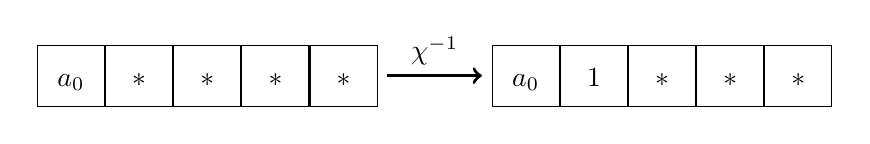
\begin{tikzpicture}[ampersand replacement=\&]
\matrix (m1) [matrix of nodes,
nodes={inner sep=5pt,text width=0.5cm,align=center,minimum height=.5cm, draw,text height=1em,text depth=.2em}
]{
	$a_0$ \& $*$ \& $*$ \& $*$ \& $*$\\
};

\matrix (m2) [right = 1.2cm of m1, matrix of nodes,
nodes={inner sep=5pt,text width=0.5cm,align=center,minimum height=.5cm, draw,text height=1em,text depth=.2em}
]{
	$a_0$ \& $1$ \& $*$ \& $*$ \& $*$\\
};
\draw[->, very thick] (m1)-- node[above, pos=0.5] {$\chi^{-1}$} (m2);
\end{tikzpicture}
\end{center}
\caption{Computation of $\chi^{-1}$\label{chi_inv2}}
\end{figure}
    \item Here in Fig. ~\ref{chi_inv2}, we fix the lane adjacent to 6th green lane as $1$ before $\chi$ operation. If this is assumed then the 6th lane is inverted as it is and seems like a constant.
    \item No. of variables : 5 lane variables + 2(substitute for quadratic terms) and 7 ( 6 linear + 1 constant) conditions. So we have Linear structure : $(A[0,0], A[0,1], A[2, 0], A[2,1], A[4,0])$
    \item White lane (constants) : 5 lanes and $64*3$ bits from $\alpha_0, \alpha_2, \alpha_4$
    \item So the degree of freedom is much larger than required 384 bits.
    \item We just want a solution with last bit of $A[2,2]$ being 1.
    \item Time complexity = $2^{384 - (64*5) + 1} = 2^{65}$
    \item If this turns out to be correct then we have a much better attack than proposed by us in our indocrypt-2018 paper with complexity of $2^{88}$
    \item We indeed have 7 variable lanes and 7 conditions.
    \item However, two of them are now artificial, and genuine number of freedom degrees is still 5. Thus we need about $2^128$ trials to satisfy the 7 conditions. Hence this doesn't work.
    \item Complexity here is $= 2^{65*\text{number\_artificial\_degree}} $
    \item But still this is our own solution for the complexity $2^{130}$.
\end{enumerate}

\subsection{Keccak-512, 1R}
\begin{enumerate}
    \item The idea is based upon linear structures though they are used for more no. of rounds but I will be using them for 1 Round.
    \item Here we linearize Keccak-f permutation for 1 round.
    \item The Preimage attack using linear structures depends directly on the space size of the variables of the linear structures formed below.
    \item d $=$ No. of output bits and $c = 2*d$
    \item $d = 512$, $c = 1024$
    \item $r = 1600 - 1025 = 576$
    \item For the Message : we keep columns 0, 1, 2 and 3 as variables
    \item \[ A[0, 1] = A[0, 0] \oplus \alpha_0 \]
        \[ A[1, 1] = A[1, 0] \oplus \alpha_1 \]
         \[ A[2, 1] = A[2, 0] \oplus \alpha_2 \]
         \[ A[3, 1] = A[3, 0] \oplus \alpha_3 \]
    \item Keep A[4,0] as constant
    \item Here $\alpha_0, \alpha_1, \alpha_2, \alpha_3$ are random constants
    \item After $\theta$ the state is only affected by constants.
    \item The $\rho$ step only rotation in lane. [Still the variables remain same]
    \item After $\pi$ step, the variables namely $(A[0,0], A[1,0], A[2,0], A[3,0])$ are shifted to different lanes.
    \item This was going forward. We have a linear structure after the above steps.
    \item Now going backward, invert $\iota$ from the hash.
    \item Invert the first 320 bits of hash by $\chi^{-1}$ i.e. the first row of hashes.
    \item We have $4*64$ free variables.
    \item So, we have a complexity gain over bruteforce of $2^{4*64}$, i.e., $2^{512 - 256} = 2 ^{256}$.
    \item Attack complexity of $2^{256}$ for 1R, Keccak-512.
    \item Verification : The Degree of freedom should be sufficient to expect a solution.
    \item Degree of freedom : $4*64$ ( from  $A[0,0], A[1,0], A[2,0], A[3,0]$) and $4*64$ (from $\alpha_0, \alpha_1, \alpha_2, \alpha_3$ ) and $1*64$ (from $A[4,0]$ constant lane)
    \item This sums up to be $9*64 = 576$, larger than required $512$.
    \item Note : More variable bits will result in lower attack complexity.
    \item This method works for all possible hash values.
    \item Present attack for 1R, Keccak-512 is \url{https://eprint.iacr.org/2017/1028.pdf}.
    \item The best attack complexity for the above is $2^{191}$.
    \item Note : Try to improve the above complexity.
\end{enumerate}

\subsection{Keccak-384, 1R}
\begin{enumerate}
    \item The idea is based upon linear structures though they are used for more no. of rounds but I will be using them for 1 Round.
    \item Here we linearize Keccak-f permutation for 1 round.
    \item The Preimage attack using linear structures depends directly on the space size of the variables of the linear structures formed below.
    \item d $=$ No. of output bits and $c = 2*d$
    \item $d = 384$, $c = 768$
    \item $r = 1600 - 768 = 832$
    \item For the Message : we keep columns 0, 2 and 4 as variables
    \item \[ A[0, 2] = A[0, 0] \oplus A[0, 1] \oplus \alpha_0 \]
         \[ A[2, 1] = A[2, 0] \oplus A[2, 1] \oplus \alpha_2 \]
         \[ A[4, 1] = A[4, 0] \oplus \alpha_4 \]
    \item Keep column 1, 3 as constant
    \item Here $\alpha_0, \alpha_2, \alpha_4$ are random constants
    \item After $\theta$ the state is only affected by constants.
    \item The $\rho$ step only rotation in lane. [Still the variables remain same]
    \item After $\pi$ step, the variables namely $(A[0,0], A[0,1], A[2,0], A[2,1], A[4,0])$ are shifted to different lanes.
    \item This was going forward. We have a linear structure after the above steps.
    \item Now going backward, invert $\iota$ from the hash.
    \item Invert the first 320 bits of hash by $\chi^{-1}$ i.e. the first row of hashes.
    \item We have $5*64$ free variables.
    \item So, we have a complexity gain over bruteforce of $2^{5*64}$, i.e., $2^{384 - 5*64} = 2^{64}$.
    \item Hence, a linear system of 320-bit equations.
    \item For generating a message satisfying the padding rule, we just need a solution with the last bit of A[2,2] being 1.
    \item Attack complexity of $2^{64 + 1} = 2^{65}$ for 1R, Keccak-384.
    \item Verification : The Degree of freedom should be sufficient to expect a solution.
    \item Degree of freedom : $5*64$ ( from  $A[0,0], A[1,0], A[2,0], A[2,1], A[4,0]$) and $3*64$ (from $\alpha_0, \alpha_2, \alpha_4$ ) and many from constant lanes
    \item This sums up to be larger than required $384$.
    \item This method works for all possible hash values.
    \item Don't know the state of the art for 1R, keccak-384.
\end{enumerate}

\subsection{Preimage attack on 2-round Keccak-256}
\begin{enumerate}
    \item \textbf{Note :} This subsection contains my explaination for the attack mentioned in section 6.1 from paper : Linear Structures: Applications to Cryptanalysis
of Round-Reduced Keccak.
    \item The message here is in lanes (0, 0), (0, 1), (0, 2), (2, 0), (2, 1), (2, 2).
    \item Keep the sum of variables in column 0, 2 constant by choosing the sum of variables in a column to be $\alpha_0 $ and $\alpha_2$ resp as constants.
    \item $d = 256 \rightarrow 4$ lanes.
    \item $c = 512 \rightarrow 8$ lanes.
    \item We can get 4 linear equations on the input bits given 4 output bits of the 5-bits.
    \item Therefore, we need 4 variables in our state to build a linear system of 256-bit equation.
    \item We have $h_0, h_1, h_2, h_3$  hash lanes in the output.
    \item By using property of $\chi$, we can get 4 linear equations on the input to the $\chi$ when 4 output bits are given.
    \item The above is true for each lane in row 0. i.e. we can get $4*64$ linear equations on the input to the $\chi$.
    \item So in one slice, we need 4 variables to map them to 4 output bits given. (according to $\chi$)
    \item So we build initial state such that we have $4*64$ free variables.
    \item So take the same structure as for 2R, Keccak-384
    \item Take $A[0, 2] = A[0, 0] \oplus A[0, 1] \oplus \alpha_0$
    \item and $A[2, 2] = A[2, 0] \oplus A[2, 1] \oplus \alpha_2$
    \item All the variable lanes will be linear.
    \item By solving the system of linear equations just once we get a solution i.e. Time complexity 1.
    \item Time complexity of attack $ = 2^{256 - 256} = 2^{0} = 1$
\end{enumerate}

\subsection{Preimage attack on 3-round Keccak-512}
\begin{enumerate}
    \item \textbf{Note :} This subsection contains my explaination for the attack mentioned in section 6.3 from paper : Linear Structures: Applications to Cryptanalysis
of Round-Reduced Keccak.
    \item We proceed as shown in section 6.1, and complete the 2 rounds.
    \item The bits input to step $\chi$ of the second round are all linear.
    \item Directly inverse 320 bits through $\chi^{-1}$ from a given hash value.
    \item Of the inverted state, each bit is a sum of 11 bits of the output of the second round.
    \item Since $\pi \circ \rho$ just permutate the positions of the bits and $\iota$ just add a constant to the first lane, they do not increase the nonlinear terms, and thus we neglect these steps in the last one and a half rounds.
    \item As in section 6.3 per equation (14) the equation of $C[x][y][z]$
    \item Expanding it :
    \item \[
        C[x][y][z] = B[x][y][z] \oplus \oplus_{y' = 0}^{4} B[x-1][y'][z] \oplus \oplus_{y' = 0}^{4} B[x+1][y'][z-1]
    \]
    \item Open all the expressions and separate two terms $B[x][y][z]$ and $B[x-1][y][z]$ and rest 9 terms remain as it is.
    \item So \[ B[x][y][z] \oplus B[x-1][y][z] = (a \oplus c + b) \oplus d
    \]
    \item Where \[
        a = A[x][y][z], b = A[x + 1][y][z], c = A[x + 2][y][z], d = A[x - 1][y][z]
    \]
    \item So guessing $d$ and other 9 terms would make $C[x][y][z]$ linear.
    \item Hence, We linearize $C[x][y][z]$ by guessing 10 bits input to step $\chi$.
    \item That is, we obtain 11 = 1 + 10 linear equations and match 1 bit of the hash value.
    \item As such, we can match $128/11 = 11$ bits of the hash value since we have 128 variables.
    \item Time complexity of preimage attack $= 2^{512 - 11} = 2^{501}$.
    \item \textbf{Note:} There is an improvement for the above attack mentioned in 6.3 by which attack complexity is $= 2^{482}$.
\end{enumerate}

\subsection{Preimage attack on 3-round Keccak-256}
\begin{enumerate}
    \item \textbf{Note} : The time complexity for attack on 3R, Keccak-256 mentioned in section 6.2 of Guo-Song-Liu paper is $ = 2^{192}$.
    \item In this method, we try to extend the structure used for preimage attack on 2R, Keccak-384 as shown in Fig. 9 of section 6.1 .
    \item For Keccak-256, $d = 256$
    \item $c = 512 = 8 $ lanes
    \item We add one more variable lane as compared to the initial state shown in Fig. 9
    \item So in Column 0, we keep $A[0,0], A[0,1], A[0,2], A[0,3]$ as variables.
    \item In Column 2, we keep $A[2,0], A[2,1], A[2,2]$ as variables.
    \item Keep \[
        A[0,3] = A[0,0] \oplus A[0,1] \oplus A[0, 2] \oplus \alpha_0
    \]
    \item \[
        A[2,2] = A[2,0] \oplus A[2,1] \oplus \alpha_2
    \]
    \item Here, $\alpha_0, \alpha_2$ are random constants.
    \item After applying $\iota \circ \chi \circ \pi \circ \rho \circ \theta $ i.e. One round the state remains linear.
    \item Input to the step $\chi$ of second round are all linear.
    \item Since we have hash of only 4 lanes, assume any random value as value of 5th lane.
    \item We can directly inverse these 320 bits through $\chi^{-1} \circ \iota^{-1}$ from given modified hash value.
    \item Then we can apply the same technique as mentioned in section 6.3 for this structure also.
    \item We linearize the $C[x][y][z]$ term as in $(14)$.
    \item As mentioned in \textbf{Improved preimage attacks on 3-round Keccak-384 and Keccak-512.}
    \item We can match $2\floor*{\frac{t - 5}{8}}$ bits of a given hash value if we have $t$ variables.
    \item For Keccak-256, we have $t = 5*64 = 320$ variables.
    \item Match bits = $78$
    \item Attack complexity $ = 2^{256 - 78} = 2^{178}$.
    \item If correct, there is a small improvement of $2^{14}$.
\end{enumerate}

\subsection{EuroCrypt'19 Keccak attack :}
\textbf{Preimage Attacks on Round-reduced Keccak -224/256 via an Allocating Approach}
\begin{enumerate}
    \item Key takeaways :
    \item Try to use two message blocks instead of one, so as to satisfy some initial conditions by xor-ing the second message block into the output state of the first block.
    \item Keep the structure simple
\end{enumerate}

\subsection{Try : Preimage Attack on Round-reduced Keccak-384 via an Allocating Approach}

\textbf{Note :} Refer mainly, \url{https://eprint.iacr.org/2019/248.pdf}

\begin{enumerate}
    \item To meet this condition : (Theorem 1)
    \item \textbf{Theorem 1 :} Let the messaged state be (a') in figure 5, i.e. bits in Row 0, 2 are unknown and bits in Row 1,3,4 are constants such that 
    \begin{enumerate}
        \item $a_{x, 1, z} = a_{x, 3, z} = a_{x, 4, z} \oplus 1$ and
        \item $\bigoplus a_{x,4,z} = 0$ 
    \end{enumerate}
    \item For Keccak-384, capacity $= 384*2 = 768 = 12 $ lanes
    \item Which means that the last 12 lanes of bits can't be changed after second message block being XOR-ed.
    \item So the last 12 lines in State (A) and (B) are identical. (refer Fig. 6)
    \item The values of the first 13 lanes in state (B) can be adjusted by second message block, to make bits in state (B) meet condition (i) and (ii) in Theorem 1.
    \item Here take state (A) of the form that variables :
    \begin{enumerate}
        \item in row 4 : $e(0,4), e(1,4), e(2,4), e(3,4), e(4,4)$
        \item in row 3 : $e(0,3), e(1,3), e(2,3), e(3,3), e(4,3)$
    \end{enumerate}
    \item It suffices to ensure :
    \item $\bigoplus e_{x,4,z} = 0$
    \item For $ a_{x, 3, z}  \oplus 1 = a_{x, 4, z}$. We ensure :
    \item $e_{0,3,z} \oplus 1 = e_{0,4,z}$,  $e_{1,3,z} \oplus 1 = e_{1,4,z}$,  $e_{2,3,z} \oplus 1 = e_{2,4,z}$
    \item $e_{3,3,z} \oplus 1 = e_{3,4,z}$, $e_{4,3,z} \oplus 1 = e_{4,4,z}$
    \item The above equations are referred as equation (3).
    \item To make bits in state (B) meet condition in theorem 1, we need $64*5 + 1 = 321$ equations to hold.
    \item Attack for keccak-384 via allocating approach, consists of 2 stages:
    \begin{enumerate}
        \item Precomputation stage : Find a first message block such that equation (3) hold for output bits of 1st block.
        \item Online stage : Construct an algebraic system using the structure in Theorem 1 for a given hash value, and solve this system for a second message block.
    \end{enumerate}
    \item Attack has 3 parts : 
    \begin{enumerate}
        \item Find a 1st message block such that equation (3) holds in precomputation stage.
        \item Find a 2nd message block such that the state (B) meets condition in theorem 1 and the outputs of the second block equal the given hash value in online stage.
        \item At last, check how to deal with the paddings.
    \end{enumerate}
    \item Part 1 : Finding a first message block
    \item Fix lanes (0,0), (0,1), (0,2), (2,0), (2,1), (2,2) as variables.
    \item Fix lane (1,0), (3, 0) as $1$ lane. Rest are $0$ lanes
    \item The state \textbf{doesnt} remain linear after 2 rounds.
    \item To find the 1st msg block satisfy equation (3).
    \item In the messaged state of 1st round, bits of 6 lanes are set as unknowns.
    \item Which means there are $6*64 = 384$ unknowns.
    \item During this procedure to avoid propagation by $\theta$ in first round, $2*64 = 128$ linear constraints are added to the system by assuming sum of linear columns as constants.
    \item The state becomes quadratic after 2 rounds.
    \item By equation (3) we obtain another 321 quadratic equations.
    \item Overall equations : $128 + 321 = 449$ in 384 unknowns.
    \item As stated in section 4.1 of this paper by Li-Sun, we use the following methods to create more linear equations : (The details are in reference with Fig 7 of the same paper)
    \begin{enumerate}
        \item Let $p_{i,j}$ be the linear representation (polynomial) of bits in state (c) of 2nd round and 
        \item $e_{i,j}$ represents the lane after 2 rounds of 1st msg block, these are quadratic variables, because before the second $\chi$ the full state was linear.
        \item By $\chi$ we have :
        \item \[
            e_{3,4} = p_{3,4} \oplus (p_{4,4} \oplus 1 ) \cdot p_{0,4}
        \]
        \item \[
            e_{4,4} = p_{4,4} \oplus (p_{0,4} \oplus 1 ) \cdot p_{1,4}
        \]
        \item By Equation (3) of same paper we have the following equations :
        \item \[
         e_{3,4} \oplus e_{4,4} = 1
        \]
        \item Hence Equation(5) 
        \[
             p_{3,4} \oplus (p_{4,4} \oplus 1 ) \cdot p_{0,4} \oplus p_{4,4} \oplus (p_{0,4} \oplus 1 ) \cdot p_{1,4} = 1
        \]
        \item Similarly, Equation (6) 
        \[
            p_{4,4} \oplus (p_{0,4} \oplus 1 ) \cdot p_{1,4} \oplus p_{4,3} \oplus (p_{0,3} \oplus 1 ) \cdot p_{1,3} = 1
        \]
        \item If the values of pair $(p_{0,3}, p_{0,4})$ are enumerated then both Equation (5) and (6) are linearized in each slice.
        \item Out of the $449$ equations only $128$ are linear due to $\theta$
        \item Get $256$ linear equations from equation 5 & 6 by enumeration for 64 slices.
        \item So no. of linear equations and unknowns match, so we can expect a solution.
        \item Actuall complexity $= 2^{449 - 384} = 2^{65}$
    \end{enumerate}
    \item The probability of existence of a solution is $2^{-65}$.
    \item The whole complexity of finding 1st msg block consists of 2 parts : Complexity $2^{65}$ of ensuring the system has a solution, and complexity constant of solving the system.
    \item Part 2 : Finding a second message block 
    \item By part 1, we get an initial state of 2nd block satisfying equation (3).
    \item For 2nd round, keep structure similar to one proposed by Guo-Song in Linear structure approach.
    \item Linear constraints by 1st $\theta$ : $2*64$ (on all columns). To avoid propagation by $\theta$ in 1st round of the second msg.
    \item Based on hash value, we can setup 320 linear equations.
    % \item 10 lanes in messaged state are unknowns. The no. of unknowns are $= 10*64$
    % \item lanes : (0,0), (0,1), (0,2), (0,3), (0,4), (1,0), (1,2), (2,0), (2,1), (2,2) are kept as variables.
    \item The system has :
    \item No. of linear equations : 2*64 + 320 = 7*64
    \item No. of unknowns = 64*6
    \item To enusre this system has a solution we enumerate $2^{64*7-64*6} = 2^{64}$
    \item So overall it will add up to $2^{66}$
    \item This is a rough bigger idea, of how to think. We need to ensure that the 2 rounds for second block are done properly.
    \item We can also make state (B) similar to the one used in (Fig 8 of paper).
\end{enumerate}

\newpage
\textbf{Key Observation }: 

In Guo-Liu-Song, Fig. 13 the (allowed) linear pattern after 32 rounds is the same as in Li-Sun, Fig. 9 (forbidden, in our view) but complexity seems $2^{192}$ rather than $2^{161}$.

\subsection{Preimage Attack on 3R, Keccak-256 using Allocating Approach}
\textbf{Note :} I refer to : \url{https://eprint.iacr.org/2019/248.pdf}
\begin{enumerate}
    \item Use the (updated image) Fig. 9 
    \item To find a first message block, we set
    \item $2*64 + 3*4 = 5*64 = 320$ linear equations
    \item By Assuming sum of linear constants in state $(a)$ and $(d)$
    \item The state after 3rd $\chi$ will be quadratic
    \item We need $e_{2,3,z} \oplus 1 = e_{2,4,z}$, $e_{3,3,z} \oplus 1 = e_{3,4,z}$, $e_{4,3,z} \oplus 1 = e_{4,4,z}$, 
    \item and $\bigoplus_{x,z} e_{x,4,z} = 1$
    \item Total $3*64 + 1 = 193$ quadratic equations to meet conditions in Theorem 1.
    \item The no. of unknowns is $6*64 = 384$
    \item So, this system consists of $320 + 193 = 513$ equations
    \item Probability of existence of a solution is $ = \frac{1}{2^{512 - 384}} = 2^{-129}$
    \item That is we need to enumerate $2^{129}$ sum values of linear columns in state $(d)$ to ensure the system has a solution.
    \item To solve : We need to enumerate the values of pair $(p_{0,3}, p_{0,4})$ in $16$ slices and obtain $64$ linear equations.
    \item Then, we obtain $64$ new linear equations and already has $320$ equations. So total $= 384$ linear equations.
    \item and then the system can be solved with a constant time complexity.
    \item Thus, the complexity of finding a first msg block $ = 2^{129 + 32} = 2^{161}$.
    \item $2^{32}$ is due to : we need to enumerate 2 variables in 16 slices i.e. 32 variables
    \item To solve a second message block, the procedure is same as that of Keccak-224
    \item Except that we obtain $4*64 = 256$ linear equations from the hash value.
    \item The System of this stage consists of : $5*64 + 2*64 0 2 + 256 = 702$ linear equations
    \item and we have $10$ variable lanes $ = 64*10 $ unknowns.
    \item We need to try $= 2^{702 - 640} = 2^{62}$ sum values of the linear columns in the state(a) of the 2nd round, to ensure that there is a solution to this system.
    \item Complexity of this stage is $2^{62}$
\end{enumerate}

\subsection{2R, Keccak-384, Internal diff}
\begin{enumerate}
    \item We start with structure of Fig. 9 initial msg in Guo-liu-song paper.
    \item To increase no. of freedome degrees we take lanes (3,0), (3,1)
    \item To keep $\theta$ constant, we are left with 5 (2 + 2 + 1) freedom degrees.
    \item Since we are performing experiment based on rotation index = 32, we assume initial msg symmetry.
    \item Hence, left with 5*32 bits of freedom degrees.
    \item We go forward with $\pi \circ \rho \circ \theta$ and get a linear state, where 2 linear lanes are adjacent. (State is still symmetric).
    \item After, $\chi$ one quadratic lane is produced. Replace this with a new linear variable of 32-bit symmetry. Since we are following rotation index property. So we artificial degree of freedom = 32
    \item So till now we have 5*32=160 actual degrees of freedom and 32 artificial.
    \item The hash state has 6 lanes. 5 lanes can be directly inverted by $\Chi$ and $\iota$. But is this symmetric?
    \item From the characteristic found of i=32, 1.5 Rounds K-384: We observe that only 3 lanes are not completely symmetric and have 3 such bits(1 from each).
    \item We initially guessed that the msg was symmetric for i=32.
    \item There are some symmetric hashes for this should work. (With some probability?)
    \item Complexity increase due to probabilistic 6th lane linear conversion will be $ = (p)^{32}$, $p = 0.75^{-1}$ due to linear for 6th lane.
    \item Complexity $ = 2^{6*32 - 5*32} * (p)^{32} $
    \item The above steps is based on what all clarity I have about the method.
    \item This should work because for lanes of our interest i.e. first 6 lanes there is hardly any difference.
\end{enumerate}

\end{document}
